\documentclass{article}
\usepackage{times}
\documentclass{article}
\usepackage{amssymb}
\usepackage{amsmath}
\usepackage{graphicx} % Required for inserting images
\usepackage[a4paper, total={7in, 10in}]{geometry}

\title{Lista 2 - MAC0320}
\author{Paulo Henrique Albuquerque, NUSP $=12542251$ }
\date{}

\begin{document}

\maketitle

\textbf{E6.} 
\vspace{5mm}

\textbf{Solução.} 



\end{document}


\title{Sistemas de arquivos \\ {\large \color{red}Notas do capítulo 5}}


\begin{document}

\maketitle

\section{Introdução}
Os três requisitos para armazenamento de informação a longo prazo são:

\begin{itemize}
  \item Deve ser possível aramazenar uma grande quantidade de informação.
  \item A informação deve sobreviver à terminação do processo usando-a. 
  \item Múltiplos processos devem ser capazes de acessar a informação de forma concorrente.
\end{itemize}

A solução usual para todos esses problemas é armazenar informação em discos em unidades chamadas \textbf{arquivos}. A informação presente nessas unidades precisam ser \textbf{persistente}, ou seja, não deve ser afetada por criação ou terminação de processos.

Arquivos são gerenciados pelo sistema operacional. A parte do SO responsável por esse gerenciamento é conhecido como o \textbf{sistema de arquivos}.

\subsection{Arquivos}

\subsubsection{Nomes de arquivos}
Arquivos são abstrações. Eles são uma forma de armazenar informação em diso para ser lida depois. Isso deve ser feito de forma que o usuário não precise se preocupar dos detalhes de como a informação é armazenada e como discos funcionam. Uma das características mais importantes de um \textit{mecanismo de abstração} é como os objetos são nomeados. Examinemos como arquivos são nomeados nos diferentes sistemas de arquivos\dots
No sistema do UNIX, há distinção entre letras maíusculas e minúsculas, MS-DOS não faz essa distinção.

O sistema Windows XP tem um sistema nativo, o New Technology File System (NTFS) que suporta nomes de arquivos em Unicode. 

Em alguns sistemas, como UNIX, extensões não são forçadas. O Windows é bastante ciente das extensões dos arquivos e atribui significado para as diferentes extensões. Algo estranho nesse sistema é que, apesar das extensões serem importantes, elas são escondidas por padrão. Isso pode ser alterado.

\subsubsection{Estrutura dos arquivos}
Há três estruturas comuns para estruturar arquivos:
\begin{\begin{itemize}

    \item Arquivo como uma simples sequência de bytes. Esse é o jeito UNIX e Windows 98. O sistema não se importa com o que está no arquivo, tudo que vê são bytes. Qualquer significado é imposto por programas de usuário.  
  \item Arquivo como sequêncio de registros de tamanhos fixos. Cada registro tem um estrutura interna. As operações de leitura e escrita atuam sobre registros.
  \item Arquivo como um árvore de registros. Cada registro tem um chave, que é usada para buscas rápidas. É amplamente utilizado em mainframes ainda utilizados em grandes centros de processamento de dados.

\end{itemize}}

\begin{figure}
  \begin{center}
    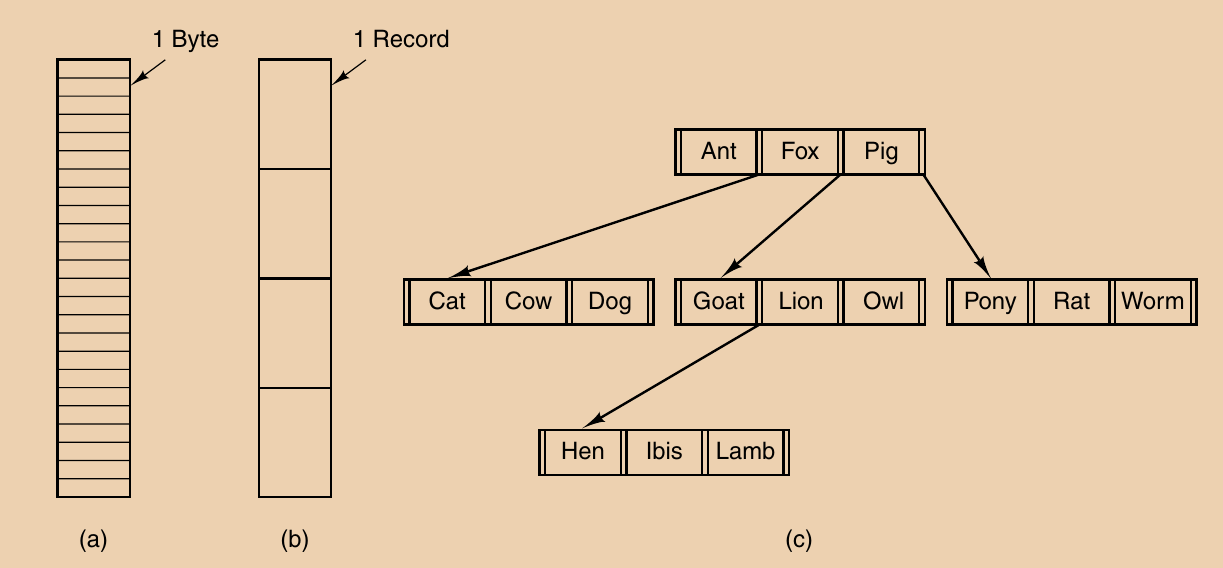
\includegraphics[width=0.95\textwidth]{img/5-2.png}
  \end{center}
  \caption{Tipos de estruturas para arquivos}
  \label{fig:}
\end{figure}

\subsubsection{Tipos de arquivos}
Há vários tipos de arquivos definidos em diferentes SO. UNIX define \textbf{arquivos regulares e diretórios}. Além de definir arquivos especiais, de bloco e de caracteres. No Windows XP há arquivos de \textbf{metadados}


\textbf{Arquivos regulares} contém informações de usuário. \textbf{diretórios} são arquivos de sistema que mantêm a estrutura do sistema de arquivos. \textbf{Arquivos de caracteres} estão relacionados a dispositivos I/O. \textbf{Arquivos de bloco} são usados para modelar discos. Estamos interessados aqui em arquivos regular e diretório, principalmente.

Em geral, arquivos regulares são arquivos texto (ACII) ou arquivos binários. Arquivos binários têm uma esrtutura interna conhecida pelos programas que os usam. 

\end{document}
